\documentclass[journal ]{new-aiaa}
\usepackage[utf8]{inputenc}
\usepackage{textcomp}
\usepackage{subcaption}
\usepackage{float}

\usepackage{graphicx}
\usepackage{amsmath}
\usepackage[version=4]{mhchem}
\usepackage{siunitx}
\usepackage{longtable,tabularx}
\setlength\LTleft{0pt} 

\title{Propellor Optimization at Different Blade Counts}

\author{Joseph Spencer \footnote{Undergraduate Researcher, Brigham Young University FLOW Lab.}}
\affil{Brigham Young University, Provo, Utah, 84601} 

\begin{document}

\maketitle

\begin{abstract}

Propellors can be modified to perform better under a variety of conditions. One project completed as part of my research for the Brigham Young University FLOW Lab explores ideal design variables for propellor performance. This investigation used computer simulations to find the optimal chord length magnification and the optimal rotation angle for a rotor's efficiency. This report defines the operating conditions used in this optimization, presents rotors that were optimized at several blade counts, and discusses areas of possible future development in this research. It found that for the operating conditions used, rotors with the chord reduced to the optimization's lower limit, 50 percent, with slight negative pitching angles were the most efficient. These results could be applied to rotors designed to produce the maximum output power for a given input power requirement, without regard to other desired outputs. Future work could combine these findings with other conditions to find the most efficient rotor that can also provide a required amount of thrust or operate at a variety of different rotational velocities.

\end{abstract}


\section*{Nomenclature}

{\renewcommand\arraystretch{1.0}
\noindent\begin{longtable*}{@{}l @{\quad \quad} l@{}}

$J$ & advance ratio \\
$\alpha$ & angle of attack (radians) \\
$\phi$ & angle of rotation (radians) \\
$M_{b}$ & bending moment (N$\cdot$m) \\
$c$ & chord length (m) \\
$D$ & diameter (m) \\
$C_{d}$ & drag coefficient \\
$\eta$ & efficiency \\
$\rho$ & fluid density (kg/m$^{3}$) \\
$v_{\infty}$ & freestream velocity (m/s) \\
$C_{l}$ & lift coefficient \\
$\theta$ & pitc angle \\
$C_{P}$ & power coefficient \\
$RPM$ & revolutions per minute \\
$\sigma$ & rotor solidity \\
$C_{T}$ & thrust coefficient \\
$C_{Q}$ & torque coefficient \\

\end{longtable*}}


\section{Introduction}

\lettrine{P}{ropellors} come in a variety of different shapes and sizes. This paper describes how one propellor, an APC 10x7 rotor\footnote{Rotor geometry obtained from the UIUC database at \url{https://m-selig.ae.illinois.edu/props/volume-1/propDB-volume-1.html}} with a NACA 4412 airfoil\footnote{Propellor geometry obtained from supporting information for CCBlade.jl at \url{https://github.com/byuflowlab/CCBlade.jl/tree/master/data}}, was used as a baseline to optimize a propellor's efficiency at a specific advance ratio. Because different blade counts could be more appropriate for different applications, blade counts of one, two, and three were each optimized and are compared in this report. This report also compares the optimized rotors of each different blade count.

Computer simulations are very useful for modeling propellors. It would require significant investment of time, space, and money to perform an optimization like this by physically propellors. In the simulation used in this report, the properties of hundreds of slightly different propellors are instead compared computationally to obtain a final result. The first potential-flow codes, programs for modeling the pressure distribution of rotors, were developed in the 1960s and 1970s. Xfoil, a program used in this project, was first developed by MIT in the 1980s, with its current version dating to 2013. Xfoil.jl was developed by Taylor McDonnell.\footnote{More information about both Xfoil and Xfoil.jl is available at \url{https://flow.byu.edu/Xfoil.jl/stable/} and \url{https://en.wikipedia.org/wiki/XFOIL}}

This paper first reviews the procedure used in the rotor optimization, including the objective function used in the optimization and the initial conditions and constraints applied. Next, it reviews the results and compares them with each other. Finally, it draws conclusions based on the results of this optimization and discusses their meaning. All code used for each section of this report can also be accessed through a GitHub repository.\footnote{This repository can be accessed in the Rotor-Design branch of \url{https://github.com/JoeSpencer1/497R-Projects/tree/Final-Report}}


\section{Methods}

Computational stimulations of propellors allow researchers to perform low-risk studies and develop designs more quickly. This project was performed using Julia programming language.\footnote{Julia is available at \url{https://julialang.org}.} Jula is available for free and is useful for a variety of reasons. Like other languages, it can easily store data in vectors and perform rapid calculations with these objects. It is compiled just-in-time with precompiled functions, which makes it run faster than interpreted languages like python without needing to be totally compiled before running like C\footnote{This article describes some of the benefits of Julia. \url{https://towardsdatascience.com/5-ways-julia-is-better-than-python-334cc66d64ae}}. Julia  packages, including those used during this semester, are also easily available from a package manager.

\subsection{Models}

Some Julia packages used for this project include Xfoil.jl,\footnote{Xfoil.jl is available at \url{https://github.com/byuflowlab/Xfoil.jl}} CCBlade,jl,\footnote{CCBlade.jl is available at \url{https://github.com/byuflowlab/CCBlade.jl}} and SNOW.jl.\footnote{SNOW.jl is available at \url{https://github.com/byuflowlab/SNOWl.jl}} Xfoil.jl analyzes the lift, drag, and moment coefficients of an airfoil from its geometry and angle of attack using a potential-flow code with a panel method. This divides the airfoil into many small surfaces and finds the lift, drag, and moment forces at each of the smaller surfaces. 

CCBlade.jl uses blade element momentum (BEM) theory.\footnote{More information about BEM theory can be found at \url{https://en.wikipedia.org/wiki/Blade_element_momentum_theory}} BEM theory, which combines blade element theory and momentum theory, calculates the axial and tangential induction factors and the angle of rotation, the angle between the free stream velocity and the tangential velocity of the rotor. After these three quantities are found, they are combined to find forces acting in all directions on the rotor\cite{CCBlade}.

The rotor in this design was created beforehand and included in the documentation for CCBlade.\footnote{Same address listed in introduction note, \url{https://github.com/byuflowlab/CCBlade.jl/tree/master/data}} Rotor data could be evaluated using XFoil.jl, but this data was selected because it had already been widened using Viterna extrapolation to include a complete range of angles of attack\footnote{Further explanation of this method is available at \url{https://flow.byu.edu/CCBlade.jl/stable/howto/}}. The airfoil polars used to analyze this are presented in the following figure. 

\begin{figure}[H]
\centering
 	\subfloat[lift coefficient]{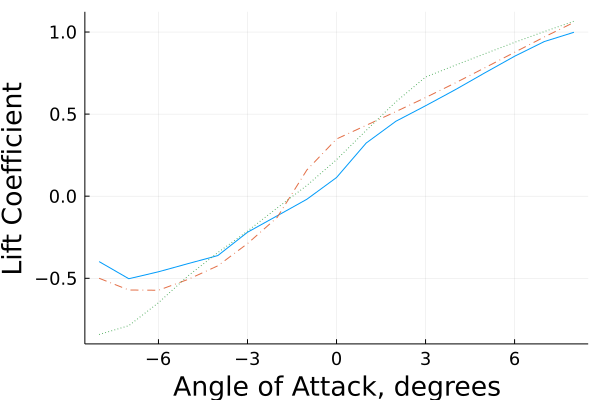
\includegraphics[width = .35\textwidth]{Plots/Figure13.png}}
	\subfloat[drag coefficient]{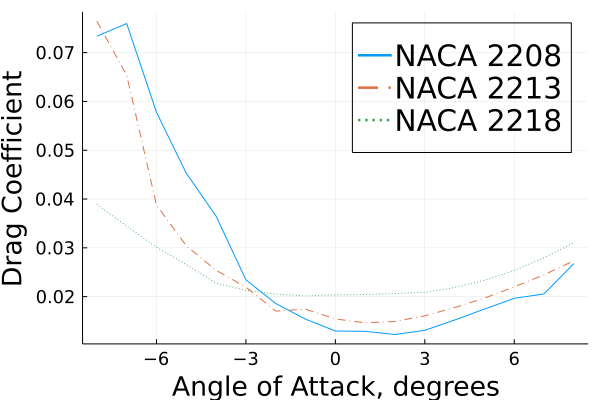
\includegraphics[width = .35\textwidth]{Plots/Figure14.png}}
	\caption{Lift and drag experienced by NACA 4412 airfoils}
	\captionsetup{aboveskip=0pt,font=it}
	\caption*{These plots show how lift and drag change for an airfoil at different angles of attack.}
	\label{fig:8}
\end{figure}

This airfoil was then placed on the APC 10x7 rotor used in the project, and its torque and power coefficients were evaluated across a range of advance ratios with CCBlade.jl. Rotors in the optimization were compared at a specific advance ratio, $J=0.472$, which is listed and explained later in this report in the bottom entry of table \ref{tab:4}. The rotor's total torque and total moment were found from the torque output of the rotor's CCBlade.jl evaluation and from integrating the normal and tangential stresses.

Once the rotor's initial torque and moment were found at this advance ratio, they were multiplied by a safety factor of $n=1.1$. This safety factor provided maximum limits for the propellor torque and moment to ensure that the SNOW.jl optimization would find the most efficient rotor that would still have reasonable input torque and power requirements to be run by the same motor and made of the same materials as the initial rotor.

In addition to restrictions on the moment and torque mentioned previously, the cord thickness was kept within a factor of two of the original and the pitching angle was kept between $-90^{\circ}$ and $90^{\circ}$. These constraints are listed in table~\eqref{equation:1} after the torque and moment constraints. They ensured that the optimization found a reasonable solution confined to realistic limits.

In this optimization, the rotor's chord length and pitching angle were modified to find the most efficient rotor. It is shown in equation~\eqref{equation:1}. 

\begin{equation}
	\label{equation:1}
	\begin{aligned}
		\mathrm{maximize:}& ~~ \eta \\
		\mathrm{with~respect~to:}& ~~ c, \theta \\
		\mathrm{subject~to:}& ~~ T \leq 1.1 T_{0};\; M_{n} \leq 1.1 M_{n0};\; M_{t} \leq 1.1 M_{t0};\; -90^{\circ} \leq \theta \leq 90^{\circ};\; 50\% \leq c \leq 200\%
	\end{aligned}
\end{equation}

Table~\eqref{tab:4} shows shared features of each of the rotors optimized. The advance ratio, $J$, is available from other variables already listed in the table by equation~\eqref{equation:3}, in which $v_{\infty}$ is the free stream velocity, $n$ is the rotational velocity in revolutions per second, and $D$ is the outer diameter.

\begin{equation}
	\begin{aligned}
	\label{equation:3}
	J = \frac{v_{\infty}}{n D} \\
	J = \frac{12}{(\frac{6000}{60}) 0.254}
	\end{aligned}
\end{equation}

\begin{center}
\begin{tabular}{| c | c | c | c |}
	\multicolumn{4}{c}{Table II: Input value limits in rotor design} \\ \hline
  	 \textbf{parameter} & \textbf{default value} & \textbf{minimum value} & \textbf{maximum value} \\ \hline
	 chord length, & 100\% length & 50\% & 200\% \\ \hline
	 pitching angle, & $0^{\circ}$ & $-90^{\circ}$ & $90^{\circ}$ \\ \hline \hline
	 rotational velocity, $RPM$ & \multicolumn{3}{c|}{6000 RPM} \\ \hline
	 blade count & 2 blades & \multicolumn{2}{c|}{1 to 3)}\\ \hline
	 hub-to-tip ratio & \multicolumn{3}{c|}{10\%} \\ \hline
	 air density & \multicolumn{3}{c|}{1.225 kg/$m^{3}$} \\ \hline
	 diameter & \multicolumn{3}{c|}{0.254 m (10 in.)} \\ \hline
	 velocity & \multicolumn{3}{c|}{12 m/s (26.84 mph)} \\ \hline
	 advance ratio & \multicolumn{3}{c|}{0.472} \\ \hline
\end{tabular}
\label{tab:4}
\end{center}

The objective function, shown in equation~\eqref{equation:1}, was optimized using SNOW.jl. SNOW.jl, developed by the FLOW Lab, finds either the maximum or minimum of a function and can intake constraint values. The code used to design the rotor was set up so that SNOW.jl found the maximum by finding the minimum of its negative. This is similar to the technique and sign convention described by Martins and Ning in \emph{Engineering Design Optimization}\cite{EngDesOpt}. SNOW.jl can also work with constraints to limit the domain of possible solutions that can be optimized, using fixed environmental variables and limits for design variables. This program used both of these types of inputs to obtain the desired solutions.


\section{Results}

Although the chord length changed during the optimization for all blade counts, the rotor's profile stayed the same throughout the optimization. It Changing the pitching angle only rotated the rotor blade, and changing the chord magnified the size of its entire profile uniformly along its entire length. The rotor and airfoil themselves retained the same shape and identification numbers throughout the optimization.

Figure~\eqref{fig:5} shows that while the optimized design increased the efficiency of even the rotor with a higher blade count above the rotor pre-optimization, it dramatically decreases the thrust and torque coefficients. The efficiency at higher advance ratios also decreased. The range of advance ratios over which the rotor maintained high efficiency was also different. This means that maximizing the rotor efficiency at a single advance ratio by only changing the chord length and twist angle may require other rotor performance properties to be sacrificed.

The plots in figure \eqref{fig:5} show that the optimized efficiency was higher than the original efficiency at every blade count. This was the desired result, as stated by the optimization function in equation~\eqref{equation:1}. Figure \eqref{fig:5} shows, though, that this increased efficiency was not obtained in exactly the way expected. While the efficiency is higher, the thrust coefficient and torque coefficient are both much lower, 
















\begin{figure}[H]
\centering
 	\subfloat[Efficiency]{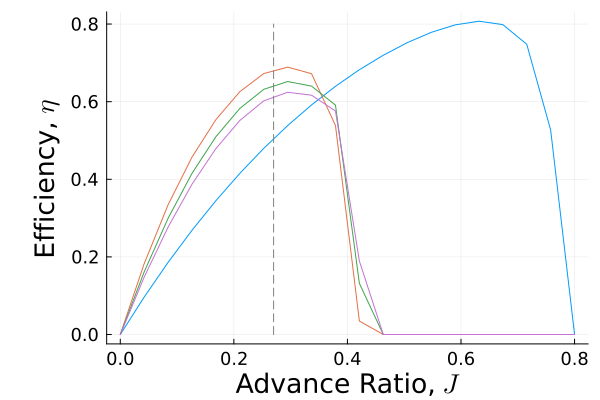
\includegraphics[width = .35\textwidth]{Plots/Figure_1.png}}
	\subfloat[Thrust Coefficient]{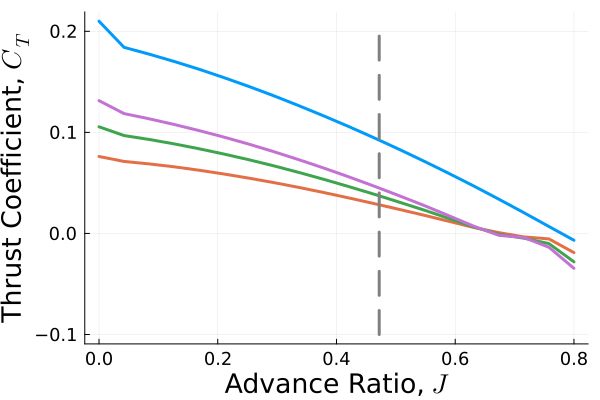
\includegraphics[width = .35\textwidth]{Plots/Figure_2.png}}

	\subfloat[Torque Coefficient]{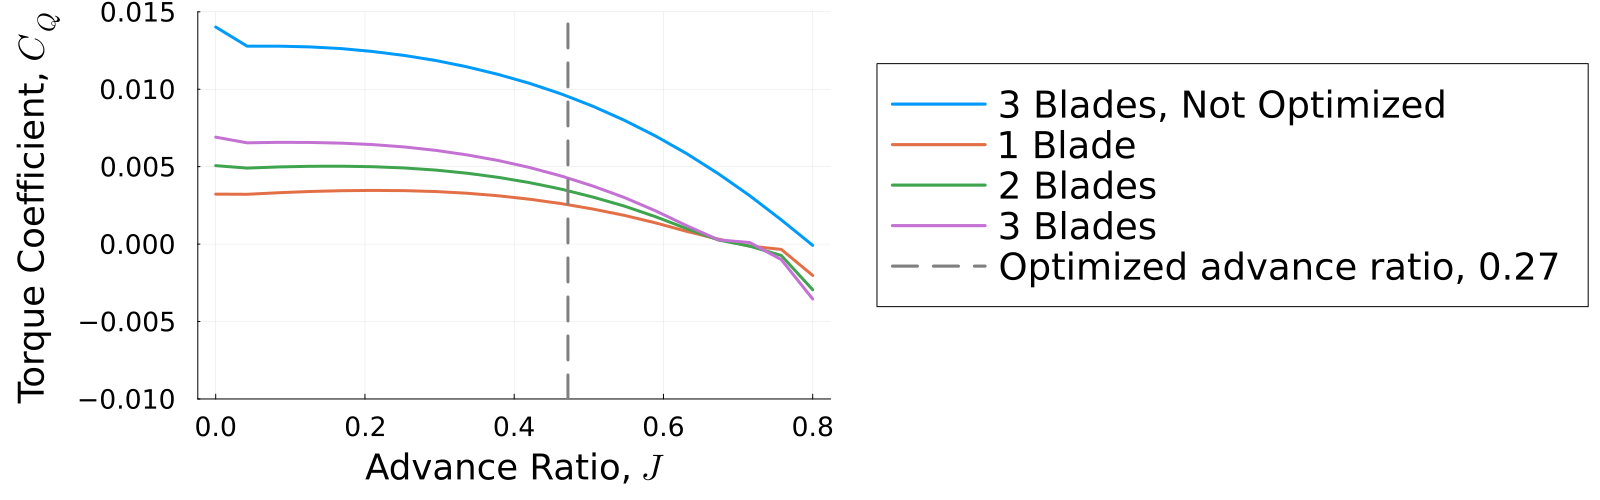
\includegraphics[width = .70\textwidth]{Plots/Figure_3.png}}\hspace{1em}
	\caption{Efficiency, Thrust Coefficients, and Torque Coefficients Compared at Different Advance Ratios}
	\captionsetup{aboveskip=0pt,font=it}
	\label{fig:5}
\end{figure}

If necessary, minimum thrust and torque coefficients could be provided as parameters along with the maximums shown below the objective function in table~\eqref{tab:2}. These could find the angle of rotation and chord length that would provide the maximum efficiency while still maintaining some required thrust. The optimizer might not reduce the rotor to its minimum possible chord length in every case as it did in this optimization.

\subsection{Results Table}

Table~\eqref{tab:6} shows the optimal pitching angles and chord magnifications for each different rotor blade count. At the conditions listed in table~\eqref{tab:4}, the optimal chord length magnification was constant, and the optimal angle of rotation was less than $-3^{\circ}$ for each rotor. It gradually became more negative as the blade count increased.

\begin{center}
\begin{tabular}{| c | c | c |}
	 \multicolumn{3}{c}{Table III (Table IV.B): Optimized chord magnification and rotation angles for different blade counts}  \\ \hline
  	 \textbf{Blade count} & \textbf{chord length Multiplication} & \textbf{Pitching angle} \\ \hline
  	 3 (Default) & 1.0 & $0^{\circ}$ \\ \hline
  	 2 & 0.50 & $-2.70^{\circ}$ \\ \hline
  	 3 & 0.50 & $-2.88^{\circ}$ \\ \hline
  	 4 & 0.50 & $-2.94^{\circ}$ \\ \hline
\end{tabular}
\label{tab:6}
\end{center}


\section{Discussion}

The propellor was checked at blade counts of 1, 2, and 3. These results found that for all three blade counts, the optimal propellor was as thin as possible, with a small negative angles of attack. The finding about thinner rotor blades being more efficient agreed with Saraf, Nouli, Ravalet, and Bakir's findings, but the negative rotation angle was surprising at first \cite{AxFlFan}.

One lesson learned from this optimization is that the user should be careful what is optimize for, because the computer will optimize exactly what it is told, even if that is not what the user actually wants. An optimization that is written incorrectly or has unseen loopholes can not only give a misleading answer but also waste a lot of time. In the case of this optimization, I think other constraints could have been added to the optimization

\subsection{Efficiency Equation}

One problem with this optimization is that a rotor's efficiency is available as a function of the advance ratio, the thrust coefficient, and the power coefficient. The equation for efficiency is described by Andrew Ning in \emph{Computational Aerodynamics}, page 200 \cite{ComAer} using the relation below, equation~\eqref{equation:7}.

\begin{equation}
	\begin{aligned}
	\label{equation:7}
	\eta = J \frac{C_{T}}{C_{P}}
	\end{aligned}
\end{equation}

With $J$ kept constant, as it was in this research, this equation can be maximized in either by maximizing $C_{T}$ or by minimizing $C_{P}$, which is equal to $C_{Q}$ multiplied by $2 \pi$. Inspection of figure~\eqref{fig:5} reveals that the optimizer did the latter. The torque coefficient $C_{Q}$ is significantly lower for each rotor. While the thrust coefficient $C_{T}$ did not decrease by as much as $C_{Q}$, it is still much lower than before. Although more efficient, the newly optimized propellor has a much lower solidity and is better suited for a different environment.

\subsection{Angle of Rotation}

The optimal angles of rotation were between $-2.70^{\circ}$ and $-2.94^{\circ}$, as shown in table~\eqref{tab:6}. These negative angles of rotation were surprising at first, because angles near $0^{\circ}$ were expected to be the most efficient. Figure~\eqref{fig:8}, from airfoil analysis conducted earlier in the semester, shows that $0^{\circ}$ angles of attack do not necessarily correspond to the lowest lift and drag coefficients for the NACA 4412 airfoil used in this design. Although that finding was for more simple analysis of an airfoil, it was concluded that a negative angle of rotation was possible.

\begin{figure}[H]
\centering
 	\subfloat[lift coefficient]{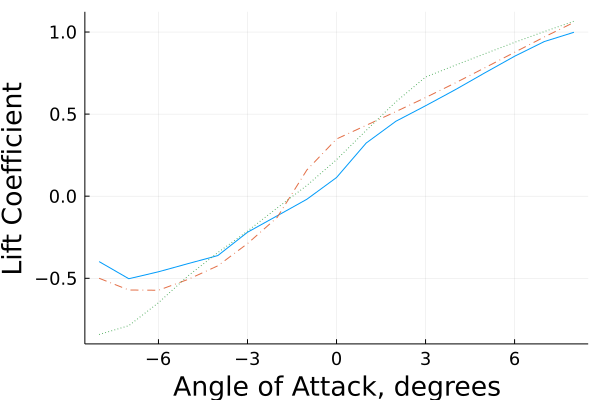
\includegraphics[width = .35\textwidth]{Plots/Figure13.png}}
	\subfloat[drag coefficient]{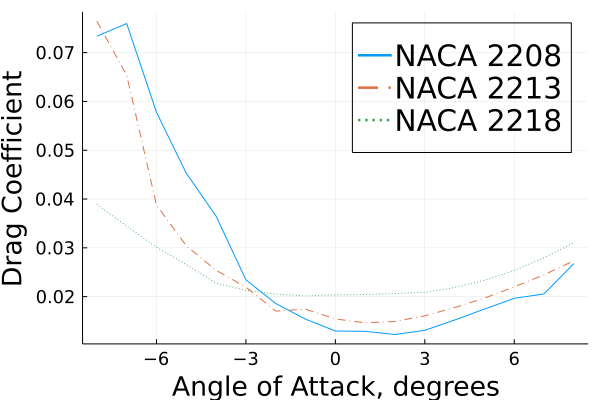
\includegraphics[width = .35\textwidth]{Plots/Figure14.png}}
	\caption{Lift and drag experienced by NACA 4412 airfoils}
	\captionsetup{aboveskip=0pt,font=it}
	\caption*{These plots show how lift and drag change for an airfoil at different angles of attack.}
	\label{fig:8}
\end{figure}


\section{Conclusion}

This optimization combined several different Julia packages to find the optimal angle of rotation and rotor chord length for a rotor's efficiency. It found that rotors with very small chord lengths at negative angles of rotation were the most efficient. Other optimizations could be performed by simple editing of the code used in this research to find which rotors perform best in other applications or environments. 


\section{Acknowledgements}

The author would like to thank Adam Cardoza for mentoring him in learning the codes used in the FLOW Lab, directing his research, helping him through questions and challenges that he discovered during his work.



\bibliography{Final_Report}

\end{document}
